\documentclass{article}
% Hyperreferences
\usepackage{hyperref}
% Margins
\usepackage[top=35mm,bottom=35mm,left=25mm,right=25mm]{geometry}
% Graphics and images
\usepackage{graphicx} \graphicspath{{./images/}}
\usepackage{subcaption}
\usepackage{float}
% Encodings (to render letters with diacritics and special characters)
\usepackage[utf8]{inputenc}
% Language
\usepackage[english]{babel}
% Section pagebreaks
\usepackage{titlesec}
\newcommand{\sectionbreak}{\clearpage}
\newcommand{\sectionnobreak}{% for when I want a section that does not break
  \global\toggletrue{afterpart}%
  \section
}
% Source code
\usepackage{listings}
\usepackage{xcolor}
\renewcommand{\lstlistingname}{File}
\lstset{
    frame=tb, % draw frame at top and bottom of the code
    tabsize=4, % tab space width
    numbers=left, % display line numbers on the left
	showstringspaces=false, % don't mark spaces in strings    
    commentstyle=\color{green}, % comment color
    keywordstyle=\color{blue}, % keyword color
    stringstyle=\color{red} % string color
}
\lstdefinelanguage{Maxima}{
	keywords={log,jacobian,determinant,subst},
	sensitive=true,
	comment=[n][\itshape]{/*}{*/}
}
% Tables with bold rows
\usepackage{tabularx}
\newcommand\setrow[1]{\gdef\rowmac{#1}#1\ignorespaces}
\newcommand\clearrow{\global\let\rowmac\relax}
\clearrow
\usepackage{multirow}
% Math stuff
\usepackage[mathscr]{euscript}
\usepackage{amsmath,amssymb}
\usepackage{mathtools}
\usepackage{enumitem}
\newcommand{\expnumber}[2]{{#1}\mathrm{e}{#2}} % scientific notation
% Definitions, theorems, remarks,...
\usepackage{amsthm}
\newtheorem{definition}{Definition}[section]
\newtheorem{theorem}{Theorem}[section]
\newtheorem{corollary}{Corollary}[theorem]
\newtheorem{lemma}[theorem]{Lemma}
\renewcommand\qedsymbol{$\blacksquare$}
\theoremstyle{remark}
\newtheorem*{remark}{Remark}
% Contents title
\addto\captionsenglish{\renewcommand*\contentsname{Table of contents}}
% Headers and footers
\usepackage{fancyhdr}
\pagestyle{fancyplain}
\fancyhf{}
\lhead{ \fancyplain{}{LabWars - Final report (LCOM 2019/20)}}
\lfoot{ \fancyplain{}{T5G03}}
\rfoot{ \fancyplain{}{\thepage} }
%
\newcommand{\email}[1]{
{\texttt{\href{mailto:#1}{#1}} }
}
\newcommand{\role}[1]{
\begin{tabular}{l l}
	\begin{minipage}[t]{30mm} \textbf{Roles} \end{minipage} &
	\begin{minipage}[t]{125mm} #1 \end{minipage}
\end{tabular}\\
}
\newcommand{\func}[1]{
\begin{tabular}{l l}
	\begin{minipage}[t]{30mm} \textbf{Functionalities} \end{minipage} &
	\begin{minipage}[t]{125mm} #1 \end{minipage}
\end{tabular}\\
}
% Metadata
\title{\Huge LabWars \\ \Large Final report \\ \vspace*{4pt} \large LCOM 2019/20}
\author{
T5G03\\
\begin{tabular}{r l}
	\email{up201806429@fe.up.pt} & Diogo Miguel Ferreira Rodrigues        \\
	\email{up201806554@fe.up.pt} & Telmo Alexandre Espirito Santo Baptista
\end{tabular}
}
\date{06/01/2020}
% Document
\begin{document}
%\begingroup
	\maketitle
%	\let\clearpage\relax
%	\setcounter{tocdepth}{2}
	\tableofcontents
%\endgroup
\section{User instructions}
\subsection{How to play}
In all game modes, the controls are the same:
\begin{itemize}
	\item \textbf{WASD} to move North, East, South and West respectively.
	\item \textbf{Mouse left-click} to fire a bullet.
	\item \textbf{Ctrl+'+'} and \textbf{Ctrl+'-'} to zoom in and out.
	\item \textbf{ESC} to escape game mode (go back).
\end{itemize}
\subsection{Main menu}
On startup, users are greeted by a \texttt{Loading...} message, briefly followed by the main screen.
\begin{figure}[H] \centering
	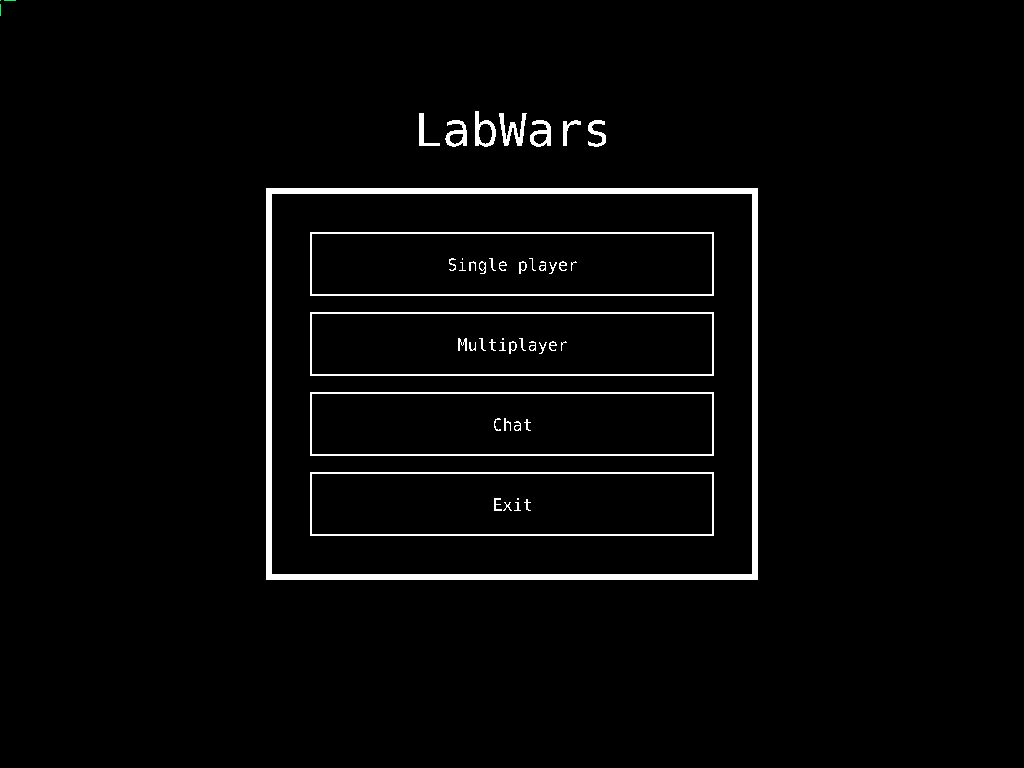
\includegraphics[scale=0.45]{main_menu}
	\caption{Main menu}
\end{figure}
Using the mouse movement and clicks, the user can select one of the avaliable options:
\begin{itemize}
	\item \textbf{Single player}: Go to single player selection menu, to select one of the single player game modes.
	\item \textbf{Multiplayer}: Go to multiplayer mode, allowing to select more options.
	\item \textbf{Chat}: Exchange text messages with another connected computer.
	\item \textbf{Exit}: Exit the game
\end{itemize}
The user can also exit the game by presing \textbf{ESC}.
\pagebreak
\subsection{Single player}
Upon entering into single player mode, the user is presented with a menu from which he can choose one of the options. \par
\begin{figure}[H] \centering
	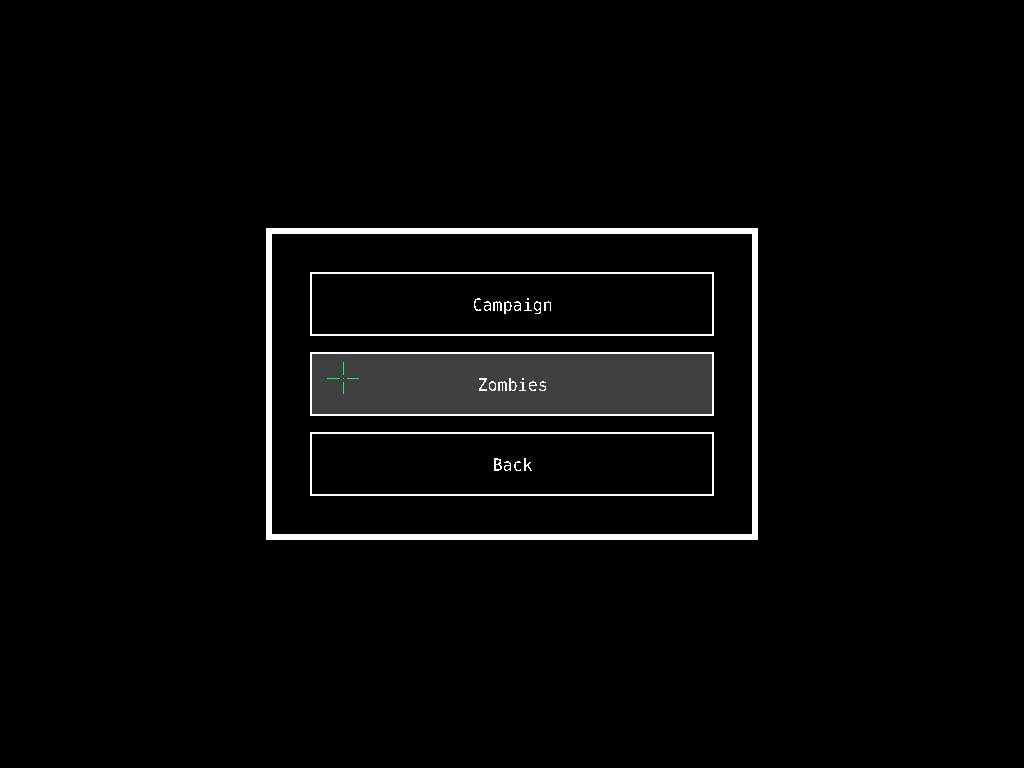
\includegraphics[scale=0.45]{singleplayer01}
	\caption{Single player menu}
\end{figure}
\begin{itemize}
	\item \textbf{Campaign}: campaign mode; kill all autonomous opponents.
	\item \textbf{Zombies}: zombies mode; kill as many zombies and survive as much time as possible.
	\item \textbf{Zombies Ranking}: Scoreboard with the highest scores obtained on zombies mode.
	\item \textbf{Back}: go back to main menu.
\end{itemize}
The user can also go back to main menu by pressing \textbf{ESC}.
\pagebreak
\subsubsection{Campaign}
In campaign mode the goal is to kill all the opponents in the map as fast as possible, while sustaining as little damage as possible.
\begin{figure}[H] \centering
	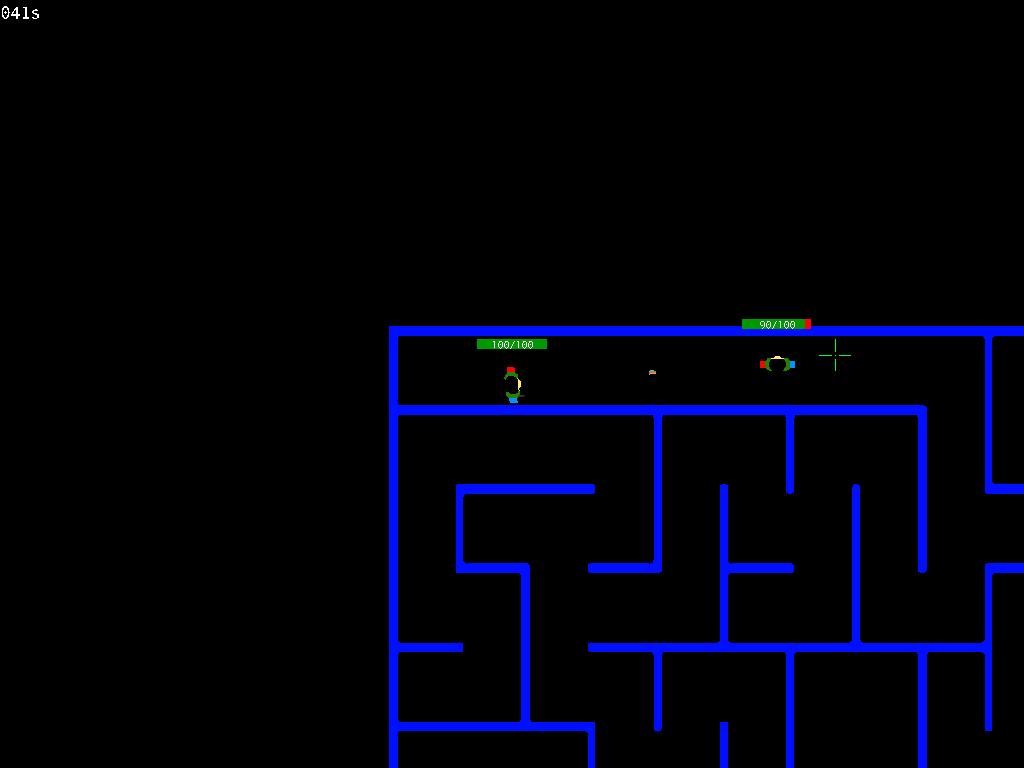
\includegraphics[scale=0.45]{campaign01}
	\caption{Campaign mode}
\end{figure}
\pagebreak
\subsubsection{Zombies}
In zombie mode the goal is to kill as many zombies and survive as much time as possible. Zombies slowly follow the player and attack the player when in short range. Once the player kills a zombie, a new zombie spawns in a random part of the map, with more life than all previous zombies.
\begin{figure}[H] \centering
	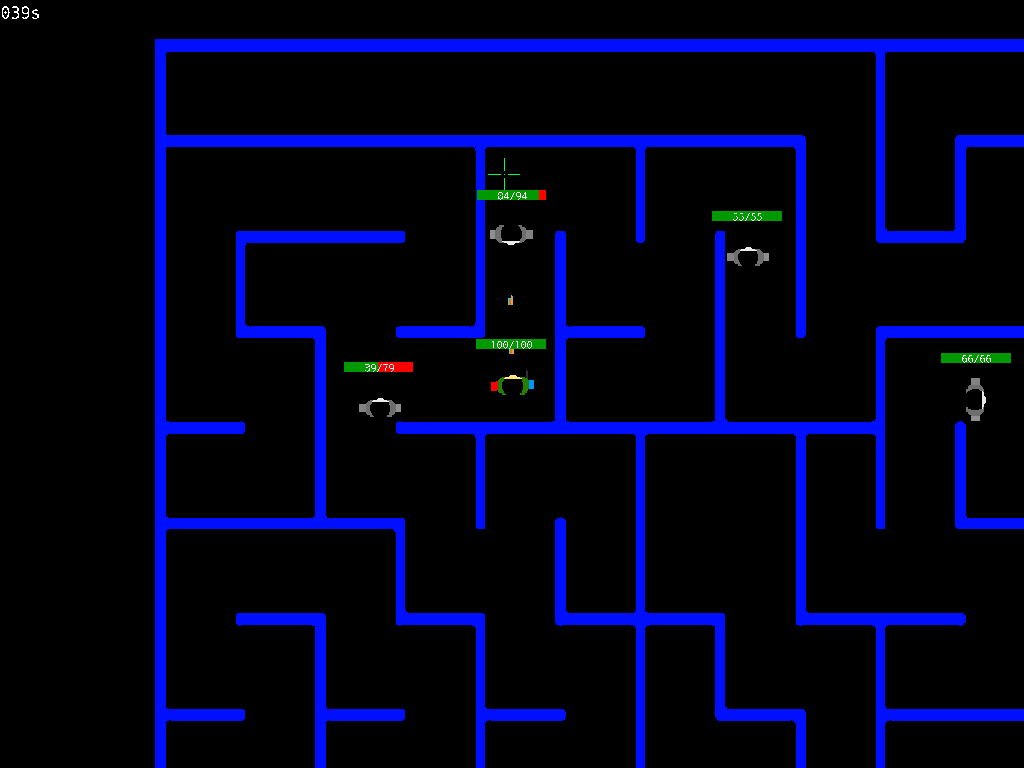
\includegraphics[scale=0.39]{zombies01}
	\caption{Zombies mode}
\end{figure}
After exiting zombie mode, the player can check the scoreboard by selecting  \textbf{Zombies Ranking}.
\begin{figure}[H] \centering
	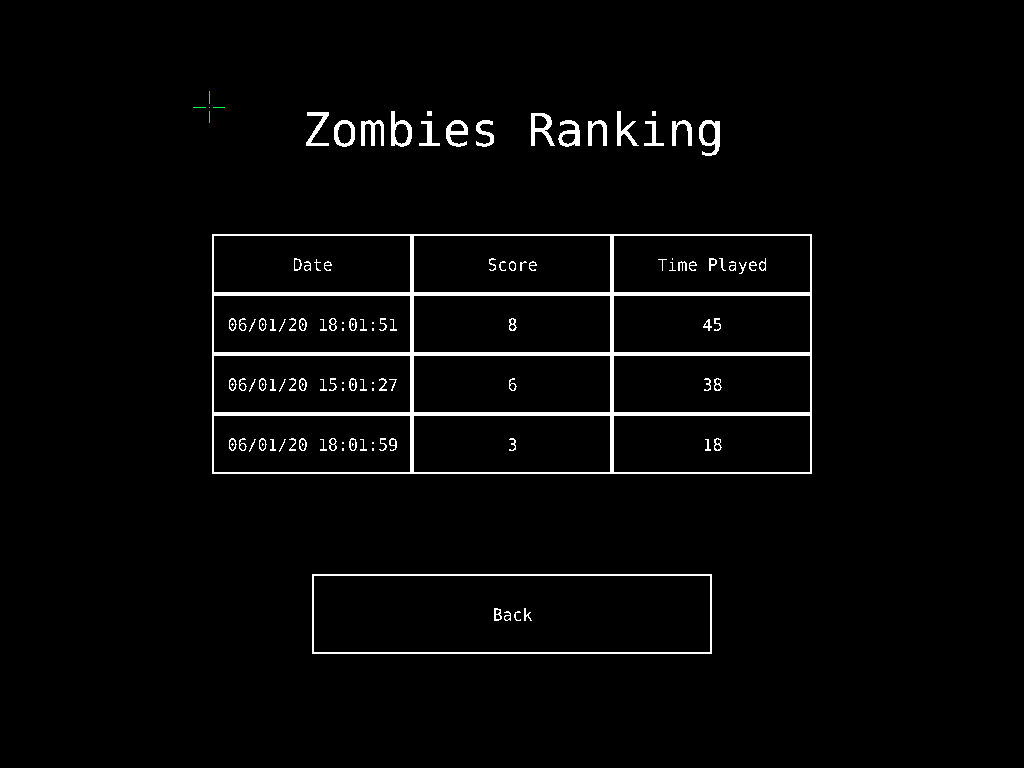
\includegraphics[scale=0.39]{zombies_scoreboard01}
	\caption{Zombies mode scoreboard}
\end{figure}
\pagebreak
\subsection{Chat}
This chat tool was initially designed as a simple, text mode, test communication between different machines. We have however decided to include it as a functionality in the project for a number of reasons:
\begin{enumerate}
	\item It was easy to develop the graphical part and integrate in the project.
	\item Having a friendly functionality that uses the communication modules allows for faster debugging; in case the computers are not properly connected, or if during development something stops working we can immediately check if the communication modules also stopped working.
	\item It served as a minimal insurance that our project would integrate the communication modules, in case we could not implement multiplayer mode.
	\item It is a useful feature.
\end{enumerate}
\begin{figure}[H] \centering
	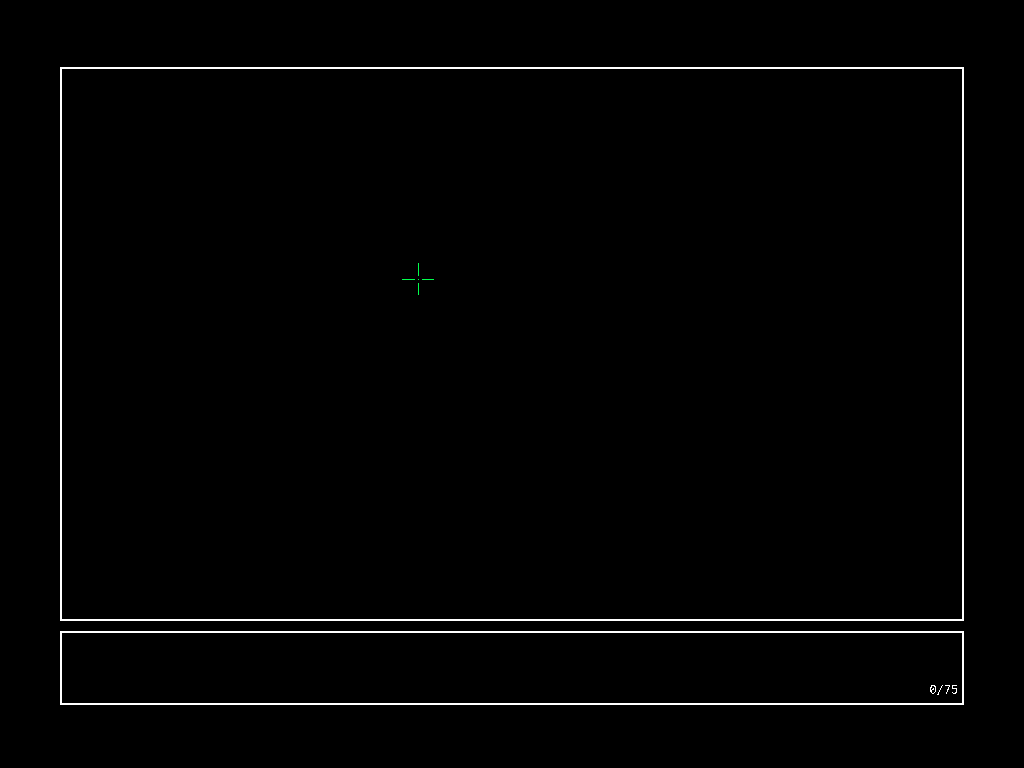
\includegraphics[scale=0.45]{chat01}
	\caption{Chat environment}
\end{figure}
The chat can be used for exchanging messages of up to 75 characters directly writable with the keyboard. The character limit was imposed to prevent strings from rendering as wider than the input box, and the fact they should be directly writable with the keyboard simplifies the process of capturing scancodes, having as downside not allowing to write characters that require more than one key press (like exclamation or question marks in a Portuguese keyboard). \par
\begin{figure}[H] \centering
	\begin{subfigure}[b]{0.48\linewidth}
		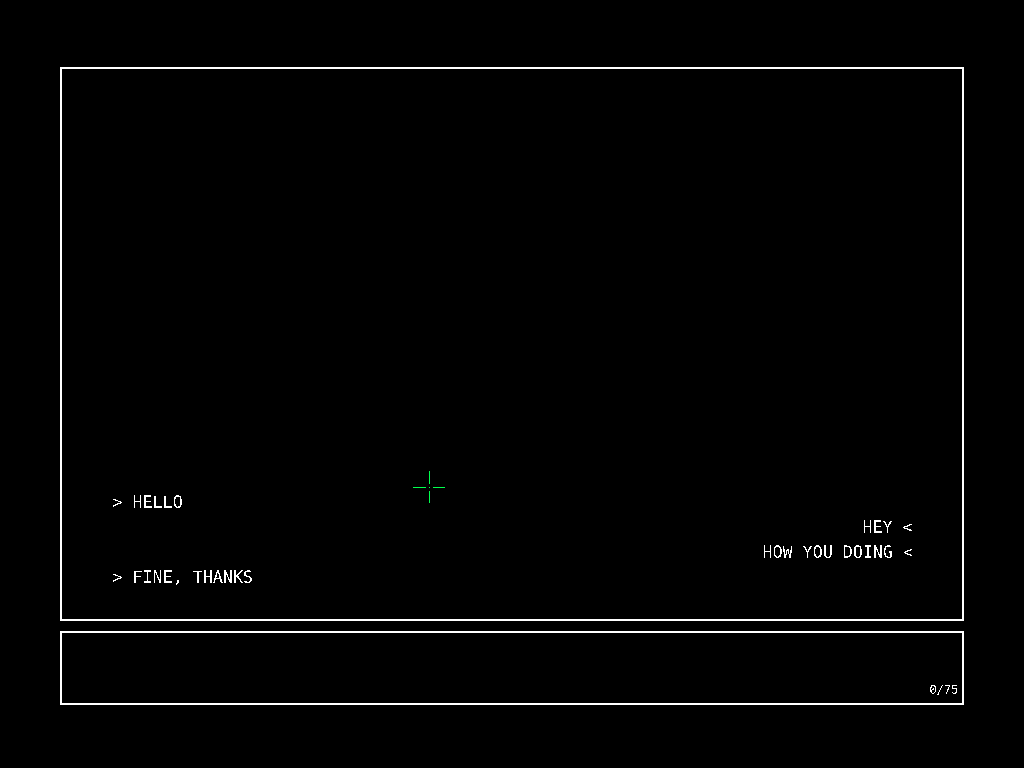
\includegraphics[width=\linewidth]{chat02_01}
		\caption{Computer 1 chat}
	\end{subfigure}
	\begin{subfigure}[b]{0.48\linewidth}
		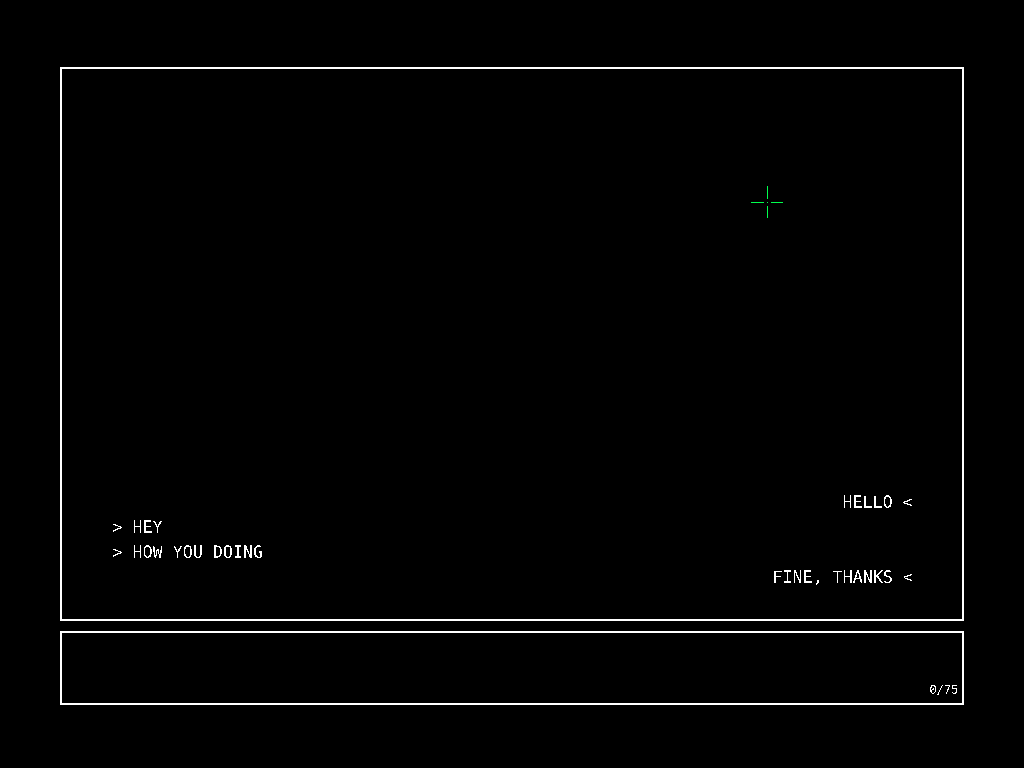
\includegraphics[width=\linewidth]{chat02_02}
		\caption{Computer 2 chat}
	\end{subfigure}
	\caption{Two users interacting via chat}
\end{figure}
The user can exit the chat mode by pressing \textbf{ESC}.
\section{Project status}
All functionalities previously presented were fully implemented, with the exception of:
\begin{itemize}
	\item \textbf{Campaign}: autonomous opponents were supposed to follow a pre-programmed path and shoot on sight at the player. Currently, they don't do either of those.
	\item \textbf{Multiplayer}: still working on it.
\end{itemize}
The I/O devices used in the project are presented in the following table.
\begin{center} \begin{tabular}{c || l | c}
	\textbf{Device} & \textbf{What for}                                        & Method \\ \hline
	Timer           & Frame rate, time since beginning of game                 & Interrupts \\
	Keyboard        & Player movement, writing chat messages                   & Interrupts \\
	Mouse           & Player orientation, shooting, selecting options in menus & Interrupts \\
	Video card      & In-game drawing, menus                                   & None \\
	RTC             & Scoreboards                                              & Interrupts \\
	Serial port     & Chat communication, multiplayer modes                    & Interrupts
\end{tabular} \end{center}
To manage all interrupt subscriptions, the general function \texttt{unsubscribe\_interrupt} was implemented and used.
\subsection{Timer}
Timer 0 is used to generate periodic interrupts at a rate of 60Hz, essentially controlling a large part of what the program does.\par
Timer interrupts regulate screen refreshing, which happens at a rate of 60Hz. In all game modes, timer interrupts serve not only the purpose of refreshing the screen, but also to process all the game data: collisions, movement, path-finding algorithms, etc. \par
To manage timer interrupt subscriptions, functions \texttt{subscribe\_timer\_interrupt}, \texttt{timer\_int\_handler} and \texttt{timer\_get\_no\_interrupts} were implemented and used.
\subsection{Keyboard}
The keyboard was configured to issue interrupts on key presses and releases. \par
The keyboard is used to control some menus (namely using \textbf{ESC}), to input text in the chat, and to control player movement in the game and zoom in/out options.\par
To manage keyboard interrupt subscription, function \texttt{subscribe\_kbc\_interrupt} was implemented. To manage keyboard interrupts, functions \texttt{kbc\_ih}, \texttt{keyboard\_get\_done}, \texttt{keyboard\_get\_scancode} and \texttt{update\_key\_presses} were implemented and used. 
\subsection{Mouse}
The mouse was configured to issue interrupts on movement and button presses. \par
The mouse is used to control all menus (position and buttons), as well as allowing the player to aim at the opponents (position) and shoot bullets (buttons). \par
To manage mouse interrupt subscription, function \texttt{subscribe\_mouse\_interrupt} was implemented. To manage mouse interrupts, functions \texttt{mouse\_ih}, \texttt{mouse\_parse\_packet} and \texttt{update\_mouse}, among others, were implemented.
\subsection{Video card}
The video card was configured to work in graphic mode with direct color encoding, with resolution 1024x768 pixels and 8 bits for each color component Red, Green and Blue, yielding a total of approximately 16.8 million colors. \par
Simple buffering was used to eliminate flickering. All graphics are first drawn to the scree buffer, and only after all graphical operations (that is, at the end of the processing of the timer interrupt) is the buffer information copied to the VRAM. \par
The modules \texttt{rectangle\_t} and \texttt{menu\_t} were developed for displaying simple shapes and menus. The modules \texttt{basic\_sprite\_t} and \texttt{sprite\_t} were developed for displaying moving sprites, allowing for rotation around the "center" of the image, as well as scaling and movement. \par
The modules \texttt{font\_t} and \texttt{text\_t} were developed to allow for dynamic rendering of text, using as default (and, for now, sole) font Consolas. The only type of supported fonts are bitmap fonts. \par
Configuration of the UART was made using the functions \texttt{graph\_init} and \texttt{graph\_cleanup} developed during the project. Drawing to the buffer is made primarily through the functions \texttt{graph\_get\_XRes}, \linebreak \texttt{graph\_get\_YRes}, \texttt{graph\_set\_pixel}, \texttt{graph\_clear\_screen} and \texttt{graph\_draw}.\par
Basic sprites are constructed from small XPM files, or loaded at runtime from XPM2 files. A XPM2 file is a XPM file stripped from all the C syntax, leaving only the strings. This format is easier to load at runtime than XPM. A XPM file can be easily converted to a XPM2 file using the function \texttt{xpm\_save\_as\_xpm2}. All XPM arrays of strings are loaded to bitmaps using the function \texttt{xpm\_load} provided by the LCF.
\subsection{Real-Time Clock (RTC)}
The RTC was configured to issue interrupts and if the interrupt source is an Update Event, in which the bit 4 of Register C will be set, then the values of time will be updated by reading their registers.\par
The date isn't updated unless asked, this is, on the interrupt notification the date isn't updated, and the reading process is different from the time. If it's asked to read the date then the date registers will be read two consecutive times, and will repeat the process if the date values of consecutive readings isn't equal, this ensures the values read are correct in case any update occurs. These updates aren't as frequent as the time values so there's no need to update it every second.\par
To manage RTC interrupt subscription, function \texttt{subscribe\_rtc\_interrupt} was implemented. In order to enable the Update Event Interrupts, the function \texttt{rtc\_set\_updates\_int} that enables or disables the Update Events interrupts by writing to bit 4 of register B. To manage mouse interrupts, function \texttt{rtc\_ih} was implemented, that verifies if the source if from an Update Event by reading register C and verifying bit 4 and if so updates the time values (seconds, minutes and hours). To ease the process of reading and writing values to the RTC, functions \texttt{rtc\_read\_register} and \texttt{rtc\_write\_register} were implemented as general functions, while having specific functions for reading the date and time values, such as \texttt{rtc\_read\_min} among others, that use the general functions cited above.\par
The RTC is used to obtain date and time for the scoreboards on the game-modes.

\subsection{Serial port}
The UART was configured to issue interrupts for Receiver Ready and Transmitter Empty. Communication is processed with the same parameters at both ends, at a bit-rate of 9600bps, 8 bits per char, 2 stop bits. UART FIFOs are used, with  trigger level of 4 bytes per interrupt. The protocols that were developed will be discussed in section \ref{sec:details}. \par
In multiplayer mode, data is transferred from host to remote at a frequency of 60Hz, with each message having at least 24 bytes. Data transference from remote to host is made whenever needed, with each message having on average 9 bytes.
\pagebreak
\section{Code organization/structure}
\subsection{\texttt{libs}}
Collection of useful classes and functions. This module was developed with the goal of being as general and independent from \texttt{proj} as possible, although there are rare occasions where sub-modules of \texttt{libs} include sub-modules of \texttt{proj}.
\subsubsection{\texttt{classes}}
Provides classes \texttt{list\_t} and \texttt{queue\_t}. These classes achieve generality by storing pointers to \texttt{void}, which have as major disadvantage requiring the use of \texttt{free}. \par
\subsubsection{\texttt{graph}}
Provides basic elements for screen drawing, like drawing pixels, rectangles, text. Manages screen buffering and VRAM.
\subsubsection{\texttt{uart}}
Provides basic functions and the NCTP protocol for communication between computers.
\subsubsection{\texttt{utils}}
Common functions, as well as functions for handling XPMs and XPM2 file format.
\subsubsection{others}
\begin{itemize}
	\item \texttt{kbc}: Manage mouse and keyboard
	\item \texttt{rtc}: Manage RTC, get current time
	\item \texttt{timer}: Manage timer 0 interrupts and subscriptions
\end{itemize}
\subsection{\texttt{proj}}
\subsubsection{\texttt{campaign}}
Campaign mode module.
\subsubsection{\texttt{chat}}
Exchange messages with connected computer.
\subsubsection{\texttt{ent}}
One of the most important modules. Implements the most important entities, and controls their interactions.
\subsubsection{\texttt{hltp}}
Provides function to interpret and send information for the serial port.
\subsubsection{\texttt{proj\_func}}
Functions related to the game dynamics, such as updating the game state, updating movement, keys presses, game timer and building the information for serial port.
\subsubsection{others}
\begin{itemize}
	\item \texttt{interrupts\_func}: group some interrupt handling functions together
	\item \texttt{makecode\_map}: map makecodes to chars
	\item \texttt{proj\_macros}: macros used throughout the project
	\item \texttt{proj\_structures}: mostly structures for transmission via HLTP
	\item \texttt{singplayer}: simple menu
\end{itemize}
\begin{center} \begin{tabular}{c | c | c | c | p{45mm} | p{45mm}}
	& & \textbf{Weight} & \textbf{Resp.} & \textbf{Contribution DR} & \textbf{Contribution TB} \\ \hline
	\multirow{7}{*}{libs}
		& classes & 13\% & DR & Everything & - \\ \cline{2-6}
		& graph   & 10\% & DR & Most part & Some contributions \\ \cline{2-6}
		& kbc     & 2\% & TB & In labs & In labs, adapted to project \\ \cline{2-6}
		& rtc     & 4\% & TB & - & Everything \\ \cline{2-6}
		& timer   & 2\% & TB & In labs & In labs, adapted to project \\ \cline{2-6}
		& uart    & 16\% & DR & Everything & - \\ \cline{2-6}
		& utils   & 3\% & DR & In labs, most part & In labs, some contributions \\ \hline
	\multirow{12}{*}{proj}
		& campaign			& 3\% & DR & Most part & Some contributions \\ \cline{2-6}
		& chat              & 7\% & DR & Everything & - \\ \cline{2-6}
		& ent               & 10\% & DR & Everything except TB & \texttt{bullet\_t} \\ \cline{2-6} 
		& hltp              & 4\% & DR & Most part & Some contributions \\ \cline{2-6}
		& interrupts\_func  & 3\% & TB & Small contribution & Most part \\ \cline{2-6}
		& makecode\_map     & 1\% & TB & - & Everything \\ \cline{2-6}
		& proj\_func        & 9\% & TB & $1/2$ & $1/2$ \\ \cline{2-6}
		& proj\_macros      & 1\% & TB & - & Everything \\ \cline{2-6}
		& proj\_structures  & 1\% & TB & - & Everything \\ \cline{2-6}
		& scoreboards       & 2\% & TB & - & Everything \\ \cline{2-6}
		& singleplayer      & 1\% & DR & Everything & - \\ \cline{2-6}
		& zombies           & 8\% & DR & Everything & -
\end{tabular} \end{center}
\section{Implementation details} \label{sec:details}
\subsection{Object-oriented programming}
Object-oriented programming was implemented to its greatest extent possible. Classes were declared using the \texttt{typedef struct} expression, and their public methods declared in the corresponding header file, always requiring as first argument a pointer/const pointer to that class. Classes were defined in the corresponding source file, and private member functions were defined as \texttt{static}.\par
The majority of entities were encapsulated in classes.
\subsection{XPM and XPM2}
The extensive use of large XPMs by simply including them with an \texttt{\#include} directive gives rise to large executable files, besides making it harder to change the used XPMs without recompiling the project.\par
The XPM2 file format is similar to XPM, except it is stripped from all the C syntax, making it a plain text file. This file format has the main advantage of being easy to load on runtime, unlike XPM that would require extensive parsing.\par
To use the XPM2 file format, two functions \texttt{xpm\_save\_to\_xpm2} and \texttt{xpm\_load\_xpm2} were implemented; the first one to convert XPM files to XPM2 files, and the second one was used in the project to load the XPM data (as an array of C-strings) from the XPM2 file format.
\subsection{Communication protocols}
\subsubsection{Non-Critical Transmission Protocol}
NCTP was designed to encapsulate the basic UART functions that were developed, by providing a set of middle-level functions that allow communication between computers.\par
NCTP allows to send a message to another computer through the function \texttt{nctp\_send}, which sends the contents of a set of memory blocks as a single message. The first argument is the number of memory blocks, followed by an array of pointers to void denoting the beginning of each memory block, and an array of sizes, where \texttt{sz[i]} is the number of bytes of the block starting at \texttt{ptr[i]} that should be sent. On receiving, NCTP calls a user-provided function to interpret the message.\par
NCTP uses queues on transmission and receiving. When a Tx interrupt occurs, NCTP tries to send as many chars of the transmission queue as possible, and on a Rx interrupts NCTP tries to extract from the receiving register as many chars as possible, putting them in the receiving queue.\par
When a complete message is detected, the chars of the message are popped out of the receiving queue, and passed to the user-provided function for interpretation.\par
A message is composed of a header, a body and trailling filler chars. The header is a pair of bytes denoting the size of the body. Then comes the body, and finally the trailling filler chars, whose purpose is to make sure the total size of the message is a multiple of 4, to prevent problems like a number of final message chars smaller than the trigger level causing a timeout.
\subsubsection{High-Level Transmission Protocol}
HLTP fills the gap left by NCTP, by providing a way to interpret messages. For that, HLTP keeps an enumeration of all the data types it knows, and for each deta type a pair of functions for coding and decoding a message containing that data type.\par
HLTP inserts at the beginning of the body a byte indicating the data type, so the message can then be decoded on the other computer.
\subsection{Path-finding}
The implementation of the following behaviour of zombies was made using a modified version of Dijkstra's path-finding algorithm. Because running a regular Dijkstra every frame causes tremendous lag, a modification was made; for each pixel, it is known the zombie should go to another pixel. At the beginning, a complete Dijkstra is ran, and each time the position of the player changes Dijkstra is only ran in the vicinity of the player.\par
This solution does not always provide the shortest path, but is significantly more efficient and returns a working path to the player.
\end{document}
